\section{Przekształcenie otrzymanej odpowiedzi skokowej}

Uzyskaną odpowiedź procesu na zmianę sygnału sterującego z punktu pracy Upp=0.8 na Umax=1.5 przekształcono w następujący sposób:
-Ograniczono (przycięto) czas zmiany sterowania u oraz wyjścia y od chwili skoku do ustabilizowania.
-Wykres sterowania u przesunięty został o wartość początkową Upp=0.8 w dół
-Wykres wyjścia y przesunięty został o wartość początkową Ypp=2 w dół
-Wykres sterowania u i wyjścia y podzielono przez delta u=0.7

Uzyskana odpowiedź skokowa daje nam zestaw liczb s1,s2… ,która wykorzystana będzie w algorytmie DMC.

\begin{figure}[H]
    \centering
    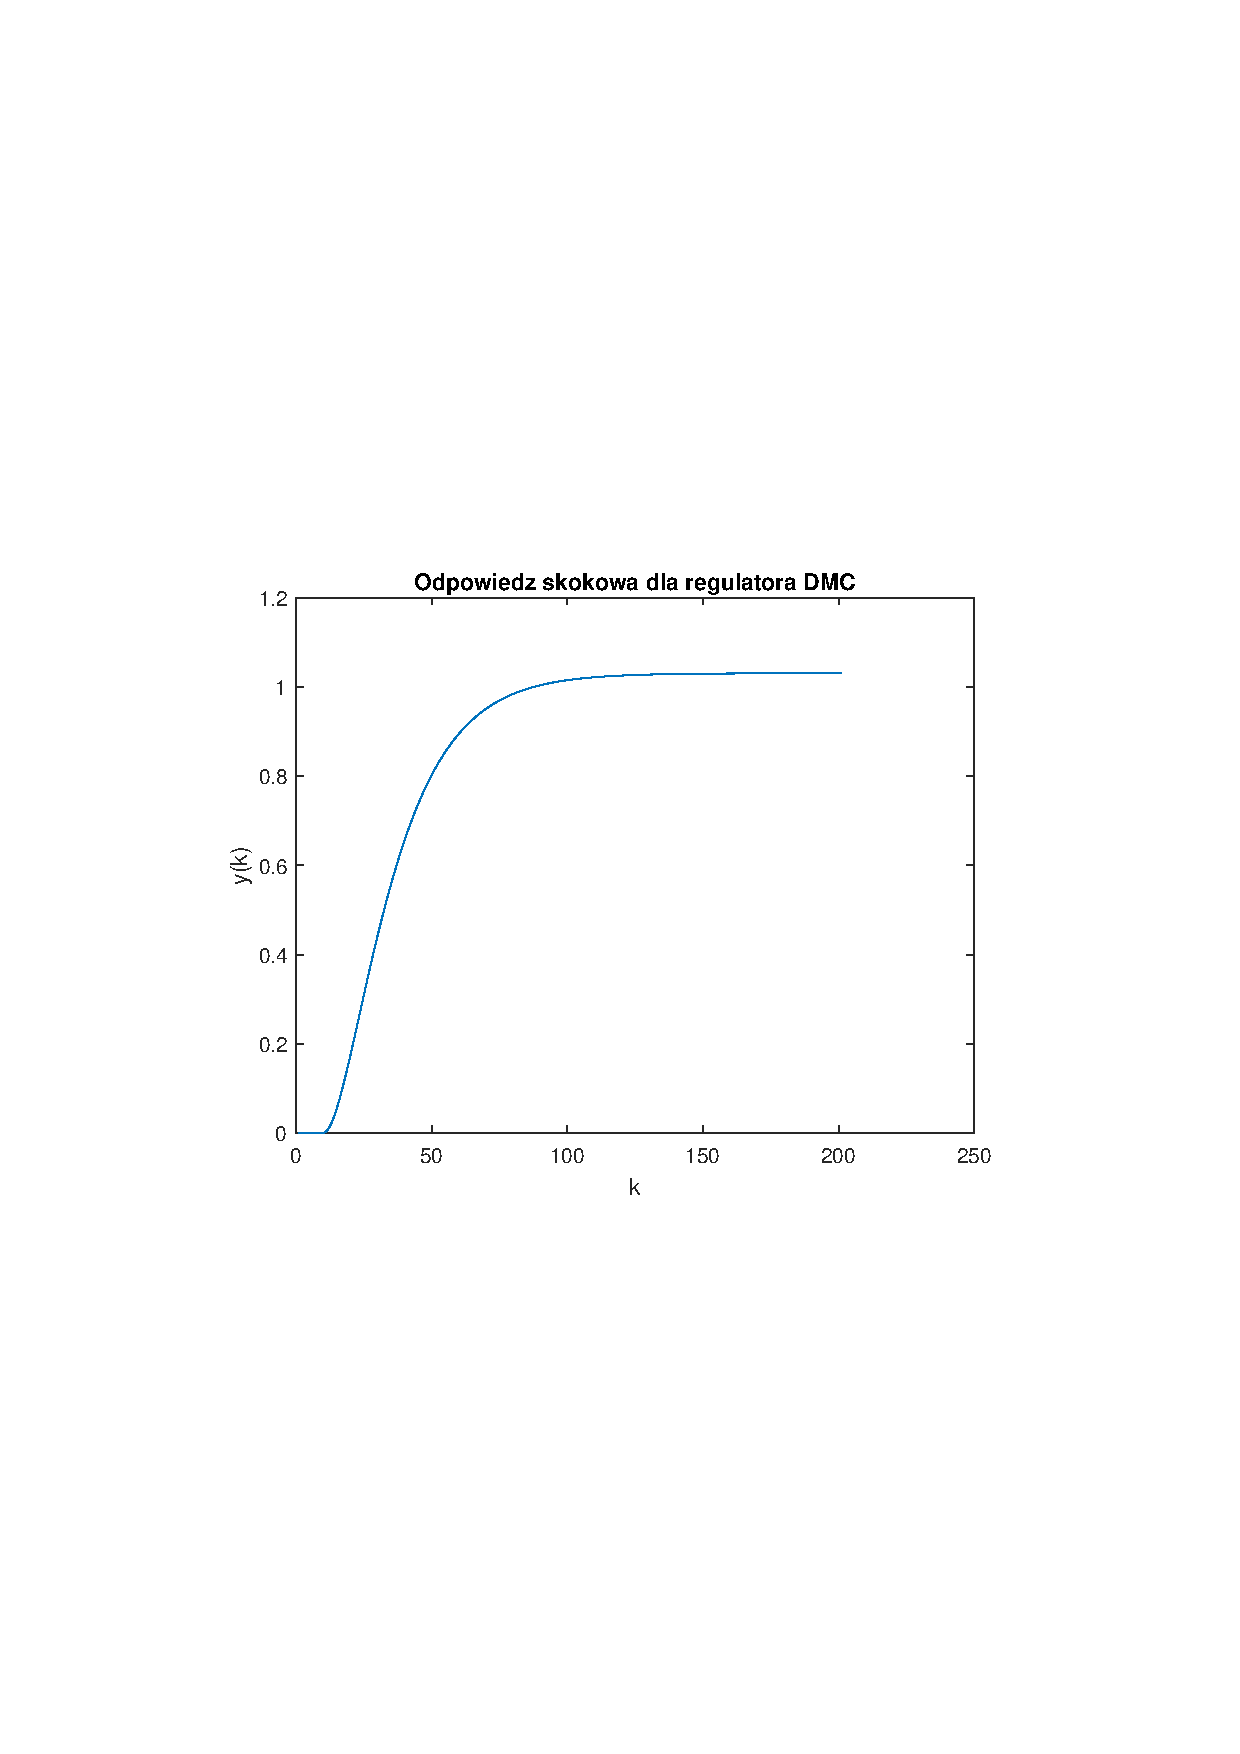
\includegraphics[scale=0.8]{../projekt/zad3/s.pdf}
    \caption{ s }
\end{figure}
